% TikZ source of grid-incidence.svg (compile with tectonic; converted with PyMuPDF, text as paths).
\documentclass[tikz,border=4pt]{standalone}
\usepackage{lmodern}
\begin{document}
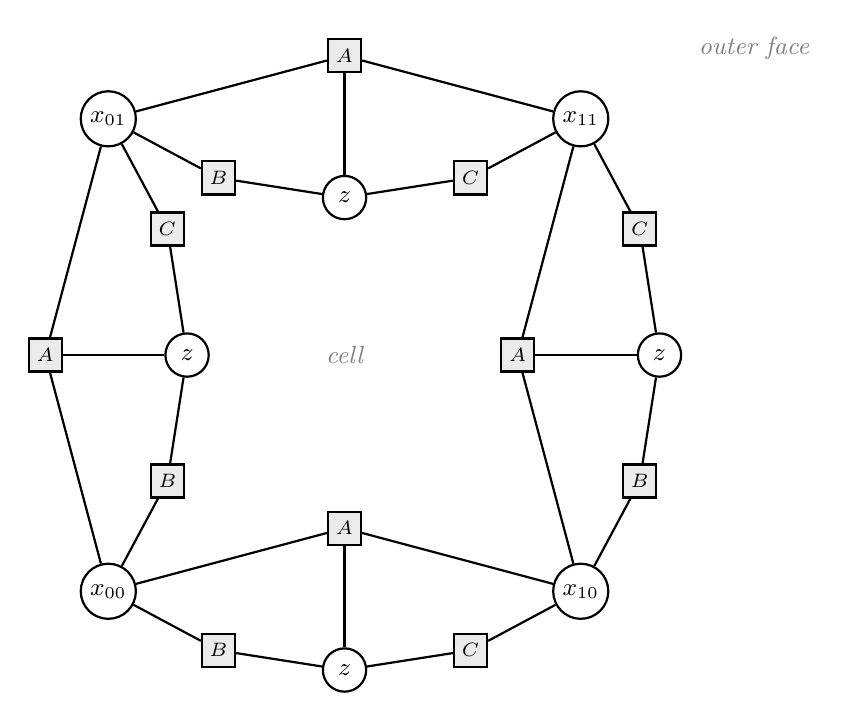
\begin{tikzpicture}[x=1cm,y=1cm,thick,
 var/.style={circle,draw,fill=white,minimum size=7mm,inner sep=0.5pt,font=\small},
 zvar/.style={circle,draw,fill=white,minimum size=5.5mm,inner sep=0.5pt,font=\small},
 clause/.style={rectangle,draw,fill=black!8,minimum size=4.2mm,inner sep=0.5pt,font=\scriptsize},
 reg/.style={text=black!50,font=\small\itshape}]
% grid points
\node[var] (p00) at (0,0) {$x_{00}$};
\node[var] (p10) at (6,0) {$x_{10}$};
\node[var] (p01) at (0,6) {$x_{01}$};
\node[var] (p11) at (6,6) {$x_{11}$};
% gadget of an oriented edge from #1 to #2; A on the left, z, B, C on the right
% bottom edge (rightward): left = above
\node[clause] (a1) at (3,0.8) {$A$};
\node[zvar] (z1) at (3,-1.0) {$z$};
\node[clause] (b1) at (1.4,-0.75) {$B$};
\node[clause] (c1) at (4.6,-0.75) {$C$};
\draw (p00)--(a1)--(p10)--(c1)--(z1)--(b1)--(p00); \draw (a1)--(z1);
% top edge (rightward): left = above
\node[clause] (a2) at (3,6.8) {$A$};
\node[zvar] (z2) at (3,5.0) {$z$};
\node[clause] (b2) at (1.4,5.25) {$B$};
\node[clause] (c2) at (4.6,5.25) {$C$};
\draw (p01)--(a2)--(p11)--(c2)--(z2)--(b2)--(p01); \draw (a2)--(z2);
% left edge (upward): left = west
\node[clause] (a3) at (-0.8,3) {$A$};
\node[zvar] (z3) at (1.0,3) {$z$};
\node[clause] (b3) at (0.75,1.4) {$B$};
\node[clause] (c3) at (0.75,4.6) {$C$};
\draw (p00)--(a3)--(p01)--(c3)--(z3)--(b3)--(p00); \draw (a3)--(z3);
% right edge (upward): left = west
\node[clause] (a4) at (5.2,3) {$A$};
\node[zvar] (z4) at (7.0,3) {$z$};
\node[clause] (b4) at (6.75,1.4) {$B$};
\node[clause] (c4) at (6.75,4.6) {$C$};
\draw (p10)--(a4)--(p11)--(c4)--(z4)--(b4)--(p10); \draw (a4)--(z4);
\node[reg] at (3,3) {cell};
\node[reg] at (8.2,6.9) {outer face};
\end{tikzpicture}
\end{document}
